%\chapter{Introduction1}
%\minitoc \mtcskip \noindent
%\chapter{Introduction2}
%\minitoc \mtcskip \noindent
\chapter{Introduction}
\label{chap:introduction}
\minitoc \mtcskip \noindent

Consumer demand is growing more than ever, and with it, concerns are raised as to whether the demand can be met in a transparent and trustful way. It is difficult to know where the products we consume come from, and the processes they go through. This leads to the need of transparency in the supply chains as well as the need of an increase in their efficiency, if they are to conform to the market's needs.

%\begin{quote}
%  ``Like the Abstract, the Introduction should be written to engage the
%  interest of the reader. It should also give the reader an idea of
%  how the dissertation is structured, and in doing so, define the
%  thread of the contents.''~\cite[chap.\ Introduction]{kn:Tha01} 
%\end{quote}

%Neste primeiro capítulo ilustra-se a utilização de citações e de
%referências biblio\-grá\-fi\-cas.
%Para além de dar um exemplo de utilização de uma citação, a citação
%anterior, introduz uma referência que pode ser consultada, entre
%muitas outras referências bibliográficas
%interessantes~\cite{kn:Tha01,kn:PP05}. 

\section{Supply Chains}
\label{supply_chains}
\textbf{Supply Chains} can be found, in some form, in nearly every business, spanning many different areas of operation. Traditionally, a supply chain encompasses all the processes and activities that lead from the initial raw materials to the final finished product, as well as all the functions and services within and outside a company. A supply chain can also be defined as the network of entities through which material flows. These entities can be identified as suppliers, carriers, manufacturing sites, distribution centers, retailers, and customers \cite{Lummus2014}. Naturally, with the upstream and downstream flow of these materials and resources, comes a lot of information on them and on the processes, people and organizations they are associated with. Realistically, the  flow is not always arborescent, as there are many considerations to be taken and decisions to be made. Supply chains have multiple end products with shared components, facilities and capacities \cite{Ganeshan1995}. As a consequence, the paths taken by the resources and information are not straightforward, but interlace, diverge and converge at different points, go back and forth, as exemplified in Figure \ref{fig:supplychain_complexity}.

\todo{fcorreia: A fig 1 é tua ou veio de algum sítio? Se não for tua é importante mencionares a fonte. Em todo o caso, parece-me deliberadamente (e desnecessariamente) complexa}
\todo{fcorreia: Todas as referências a secções, capítulos, figuras, tabelas devem começar por letra maiúscula. Na referência a esta figura está bem, mas não o tens sempre pelo documento fora}
  
\begin{figure}[ht]
\centering
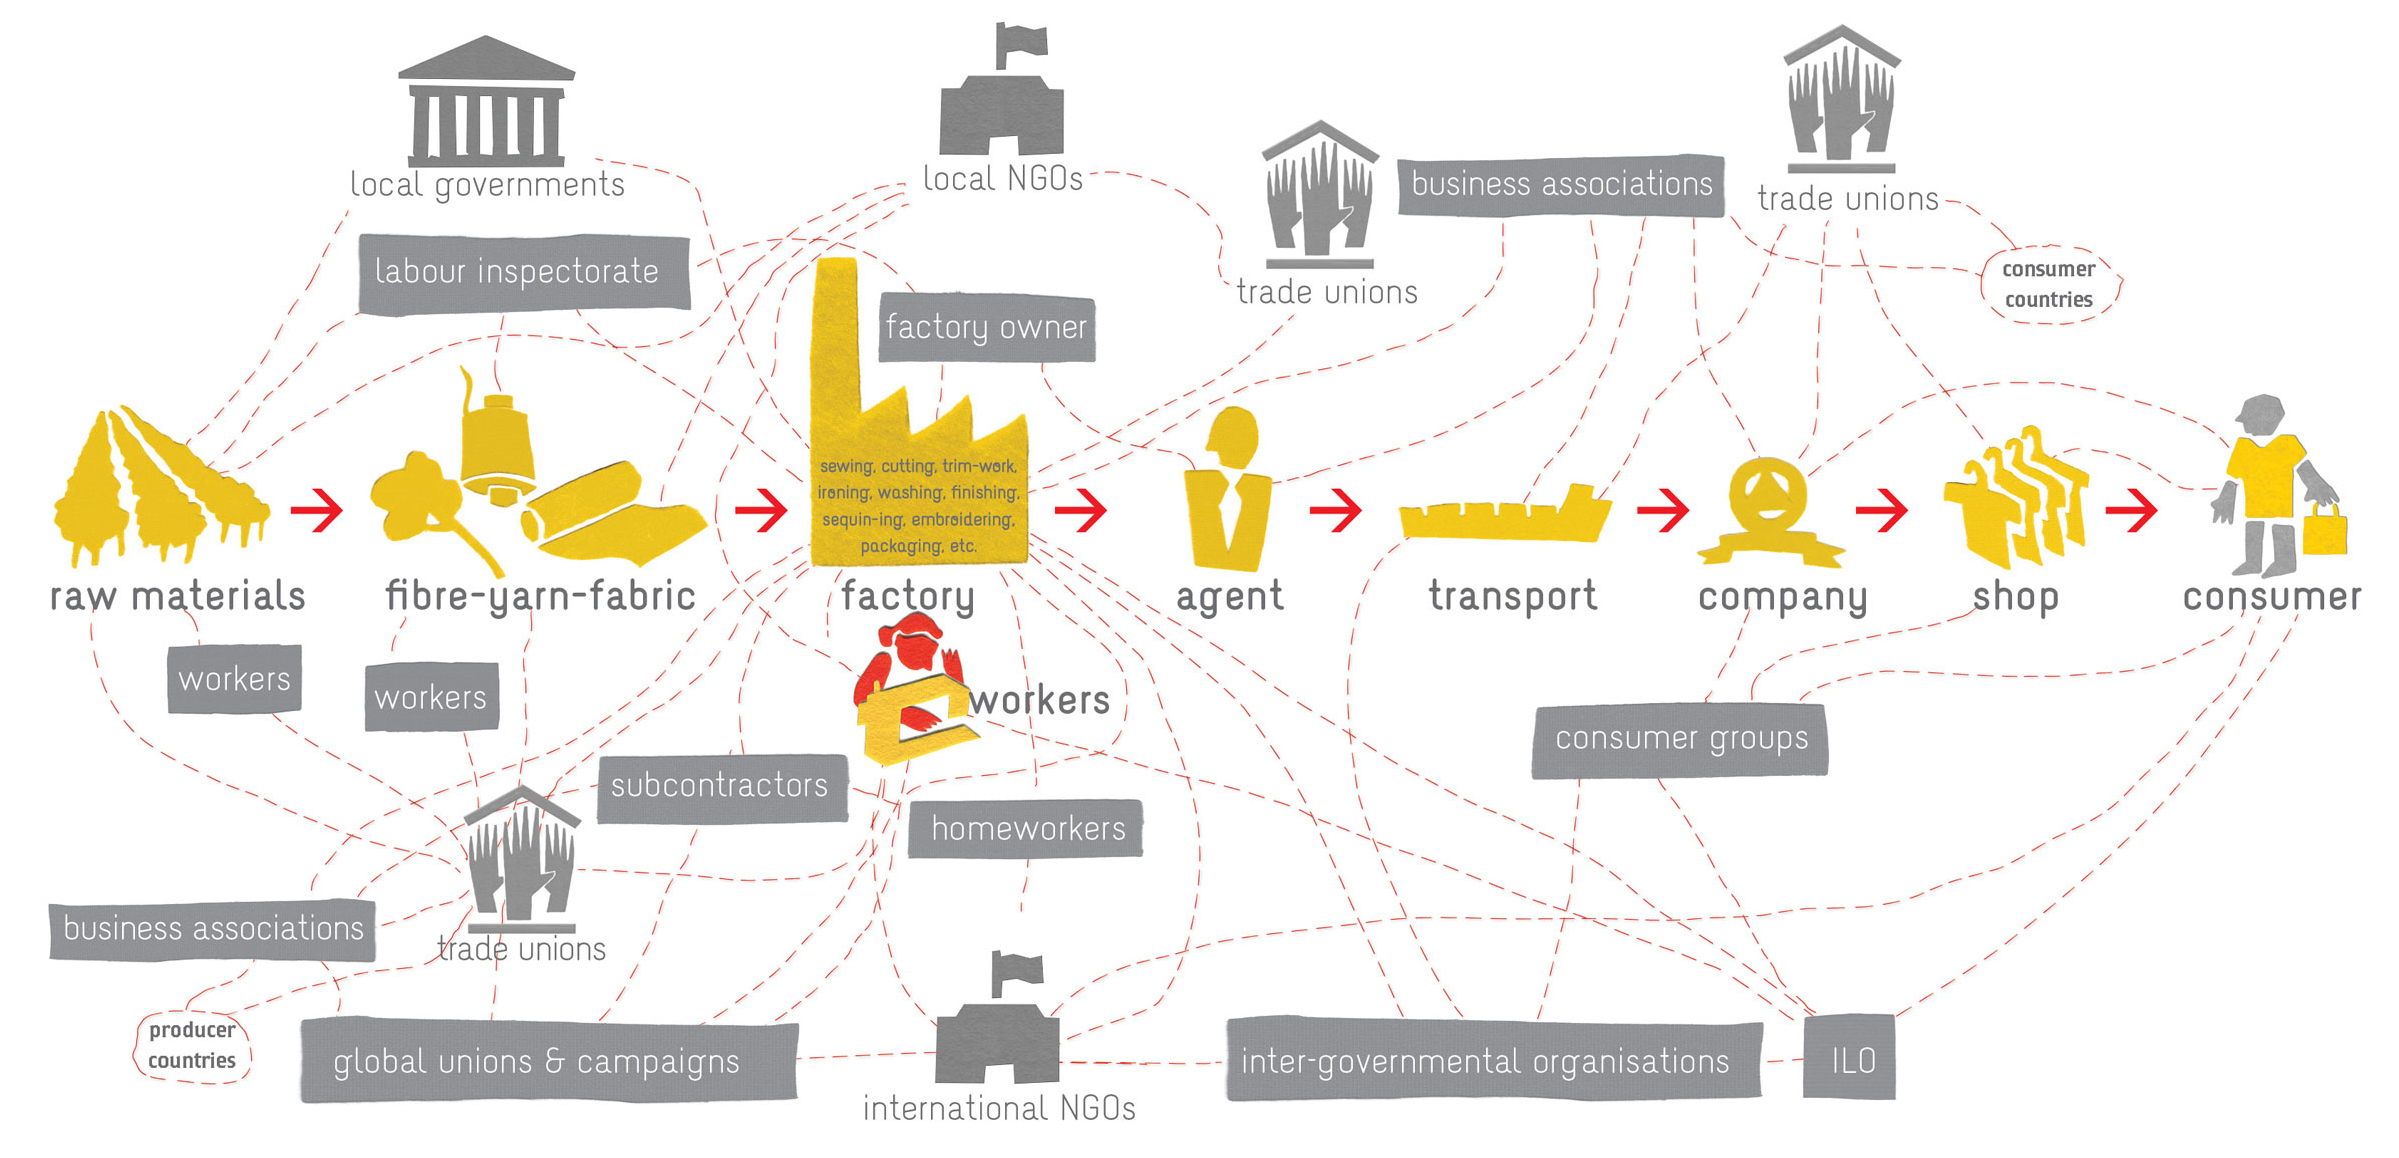
\includegraphics[scale=0.18]{media/supplychain_complexity.jpg}
\caption{Representation of a garment supply chain and all the relationships it involves}
\label{fig:supplychain_complexity}
\end{figure}
  
  The activities and processes a supply chain encompasses include: sourcing raw materials and parts, manufacturing and assembly, warehousing and inventory tracking, order entry and order management, distribution across all channels, delivery to the customer, and managing the information systems necessary to monitor all of these activities. As Lummus \cite{Lummus2014} describes, these activities can be roughly mapped to the 4 essential processes: plan, source, make, deliver.
    
  Coordinating all of these is no easy task, and so the discipline of SCM comes into life. According to Ballou \cite{Ballou2007}, the Council of SCM Professionals (CSCMP) defines SCM as \textit{“the planning and management of all activities involved in sourcing and procurement, conversion, and all Logistics Management activities. Importantly, it also includes coordination and collaboration with channel partners, which can be suppliers, intermediaries, third-party service providers, and customers. In essence, SCM integrates supply and demand management within and across companies”}.

From this definition follows that SCM deals a lot with both coordination and collaboration between entities, and so, the management of the flow of information and resources between them is very important. The objective is always, of course, to minimize the total cost of these flows between and among stages \cite{Habib2011}.
In the end, the creation of value (products and services) in a supply chain stems from the relationships that different entities build between themselves, and not from the work of a single entity. As such, supply chains, not firms, compete and those which have the best integration and management processes win.

And this is where SCM shines and shows just how useful it can be. Managing all the processes in a supply chain, while maintaining safety, quality and keeping to schedule is difficult. An event on one side of the world, large or small, be it from human or natural causes, can easily disrupt the links in the supply chain. For instance, it might disrupt the supply of a critical component or service. Delays are, therefore, common, and the consequences of such disruptions might have a severe impact in the finances, growth and reputation of the companies involved \cite{Punter2013}.

SCM diminishes the impact of such disruptions, and actively works to avoid or diminish them, while optimizing the way the supply chain works. This is why SCM is such an important discipline, that we have to better understand and improve, with all the means that we can, and this includes, of course, technologies like the blockchain.

\section{Challenges}
\label{supply_chain_challenges}

 Having already introduced the concepts of Supply Chain and SCM, it is now possible to briefly introduce some of the problems that affect them.

The first, and most generalist problem of a supply chain, is the ease with which \textbf{an unexpected event might cause delays}. These events, already mentioned in section \ref{supply_chains} are not always predictable and must be contained as fast as possible. One event in particular which, often, causes delays are \textbf{synchronization problems in the information systems of a company}. 

    Another problem is that, often, there are difficulties in sharing information between companies. This is caused both by the fact that \textbf{companies value their privacy and the security of their information}, which means they might not want to share too much information, or that they might only share it through secure channels, and by the \textbf{lack of standards for sending information and communicating} \cite{Korpela2017}. The issue with non-existing standards is that companies are left to discuss what details to share or not, wasting time and resources.

Most important of all, in the industry, \textbf{the use of traditional tools and manual work is still too prevalent}. Emails are sent, documents are printed and mailed, instead of transmitting the information in a more automatic, direct and secure way through the network. This point also brings the next problem of supply chains to light: the apparent lack of interoperability between certain softwares (which might be a byproduct of by the lack of standards).
 
 %talk about payment processing, such as to introduce smart contracts later?
 
Finally, provenance and traceability of the products on a supply chain are a big objective for companies. But \textbf{the current technologies used in supply chain only accomplish provenance and traceability in a limited scope}, as the information a certain entity possesses is usually also limited. And so, it is very hard for anyone to have a global overview of the supply chain.

Most of these issues in supply chain are, in part, caused by the standalone use of outdated or inadequate software architectures, which are often centralized and have single points of failure. An optimal supply chain should be as efficient and effective as possible, while being secure and satisfying all the traceability requirements. Perhaps, it is time to try out new solutions which replace or complement the existing ones, in a way that supply chain management can better satisfy these requirements.

\section{From Blockchain Technologies to Supply Chains} \label{sec:context}

Blockchain technology allows for secure, public, distributed and decentralized systems. Though it was first proposed in its actual form by Satoshi Nakamoto \cite{Nakamoto2008}, an anonymous group which published a white paper in 2008, this was not the first reference to such a technology. The first work on a cryptographically secured chain of blocks was described in 1991 by Stuart Haber and W. Scott Stornetta \cite{Haber1991}, and further refined in 1992 by Bayer \& Haber, by incorporating Merkle trees \cite{Bayer1993}. Since then, it has come a long way, sprouting multiple different uses and applications of the technology. Its characteristics make the development of distributed and permanently, globally available systems possible, which is a paradigm that is attracting the interest of various industries.

One area in particular where we believe blockchain could bring about great improvements is Supply Chain Management (SCM). SCM has seen an increase in complexity in the last few decades, due to the globalization of the market, with businesses interlacing in many different ways, their relations extending way beyond what they used to, as found by Filiz Isik \cite{Isik2011}. This increase in complexity is somewhat hard to manage and some supply chains stretch and encompass so many businesses that, due to their software not being prepared for this, the information is not always transmitted from end to end, leaving holes of information in between the links that join each business, thus leading to a lot of chaos and uncertainty as to the state of the key items in the chain \cite{Wilding1998}.

   This dissertation work will focus on supply chain management, and on how blockchains can possibly be applied to improve this area, leading to positive impacts in the logistics industry and eventually finding benefits for the consumer as well. 

%Esta secção descreve a área em que o trabalho se insere, podendo
%referir um eventual projeto de que faz parte e apresentar uma breve
%descrição da empresa onde o trabalho decorreu.

%Lorem ipsum~\cite{kn:Lip08} dolor sit amet, consectetuer adipiscing
%elit. 







%%%%%%%%%%%%%%%%%%%%%%%%%%%%%%%%%%%%%%%%%%%%%%%%%%%%%%%%%%%%%%%%%%%

\section{Motivation} \label{sec:motivation}

As described in section 1.3, these problems are caused by the use of software that can't keep up with the evolution of the supply chains. It is either outdated or inadequate software by itself, and even when the software works just fine, it wasn't specified to allow for the integration of a whole chain. There is an immediate need for better solutions. New and better solutions might not completely replace the previous ones, but, rather, add to them.

One way to approach these specific problems that are caused by the traditional IT solutions is to update them with the use of new technologies, namely by taking what already exists and integrating it with blockchain technology. The characteristics of blockchain would allow for many of the identified problems to be reduced or neutralized. Blockchains are the perfect means to achieve traceability of a supply chain, and so, they are good to achieve provenance as well. At the same time they are a secure, incorruptible and immutable way to store information, with a fast synchronization time, being perpetually available to anyone who has permission, anywhere within the network. It would also be the way to close the analog gaps, turning the chain fully digital, leading to the possibility of a global overview.

\section{Objectives}
\label{sec:objectives}
The main objective of this dissertation is to find whether blockchain technology can really solve the most common problems of supply chain management, and in which areas of SCM it could help out the most. There are a multitude of small tasks that blockchain could automatize in supply chain, so this thesis will try to figure out which ones blockchain applies to better. 

Certain designs are going to be proposed, with focus on different issues and giving solutions to different archetypes of supply chains and integration models. As a secondary objective, we are going to find which design better fits in order to build a generalist solution to our problem and also what are the requirements for blockchain to be applied in this sense.

\section{Dissertation Structure} \label{sec:struct}

%TODO{Update the structure}

Besides the introduction, this dissertation has 4 more chapters. The state of the art is divided into 3 chapters: \ref{chap:blockchain}, \ref{chap:blockchain-frameworks} e \ref{chap:blockchain-applicability}.

In the chapter~\ref{chap:blockchain}, some important Blockchain concepts are introduced, which are crucial to understanding the rest of the content. In the chapter~\ref{chap:blockchain-frameworks}, the most relevant Blockchain development platforms are described, such as Ethereum and Hyperledger Fabric. In the chapter ~\ref{chap:blockchain-applicability}, the advantages and disadvantages of applying blockchain technologies to supply chain are discussed, and some related works are shown. Still in this chapter, some important design decisions are also presented.

The last chapter, \ref{chap:conclusions}, describes the future work, along with some of the metrics that will be used to evaluate this work. It also explains what the expected results will be.


\todo{fcorreia: faltam referir/descrever aqui alguns capítulos}
